\subsection{Transfer to DEA, MDEA and AMP}\label{sec:results-transfer}
% P:transfer-parameters
With the shared parameters fixed, each of the three further amines can be fitted.
\Cref{tab:transfer-species,tab:transfer-fitted} give the parameters of the DEA, MDEA and AMP models, and Table~\ref{supp-tab:supplement-transfer-data} lists every data set with its role, ranges and deviations.

\begin{table}[pos=!htbp]\small\setlength{\tabcolsep}{2pt}\caption{Segment, association and Born parameters of the DEA, MDEA and AMP species.}\label{tab:transfer-species}
\begin{tabular}{@{}>{\raggedright\arraybackslash}p{0.12\linewidth}>{\raggedright\arraybackslash}p{0.1\linewidth}>{\raggedright\arraybackslash}p{0.1\linewidth}>{\raggedright\arraybackslash}p{0.12\linewidth}>{\raggedright\arraybackslash}p{0.13\linewidth}>{\raggedright\arraybackslash}p{0.1\linewidth}>{\raggedright\arraybackslash}p{0.12\linewidth}>{\raggedright\arraybackslash}p{0.14\linewidth}@{}}
\toprule Species & $m^{\mathrm{seg}}$ & $\sigma$ (\AA) & $u/k_B$ (K) & $\epsilon^{AB}/k_B$ (K) & $\kappa^{AB}$ & $d^{\mathrm{Born}}$ (\AA) & Ref. \\ \midrule
\ce{DEA} & $5.2048$ & $2.9477$ & $269$ & $1517.6$ & $0.1014$ & -- & \cite{Nasrifar2010} \\
\ce{DEAH+} & $5.2048$ & $2.9477$ & $269$ & $0$ & $0.1014$ & $2.9477$ & \cite{Nasrifar2010}\textsuperscript{a} \\
\ce{DEACOO-} & $1$ & $6.1672$ & $183.0006$ & -- & -- & $6.1672$ & This work\textsuperscript{b} \\
\ce{MDEA} & $3.675$ & $3.563$ & $228.711$ & $2046.624$ & $0.118$ & -- & \cite{Pahlavanzadeh2013,Uyan2015}\textsuperscript{c} \\
\ce{MDEAH+} & $3.675$ & $\boldsymbol{3.6430}$ & $\boldsymbol{596.464}$ & $0$ & $0.118$ & $3.6430$ & This work\textsuperscript{d} \\
\ce{AMP} & $\boldsymbol{4.0761}$ & $\boldsymbol{3.1870}$ & $\boldsymbol{237.0599}$ & $\boldsymbol{2385.1893}$ & $\boldsymbol{0.0366}$ & -- & This work\textsuperscript{e} \\
\ce{AMPH+} & $1$ & $\boldsymbol{5.7699}$ & $237.0599$ & -- & -- & $5.7699$ & This work\textsuperscript{f} \\
\ce{AMPCOO-} & $1$ & $\boldsymbol{6.4705}$ & $183.0006$ & -- & -- & $6.4705$ & This work\textsuperscript{g} \\
\bottomrule\end{tabular}
\par\smallskip{\footnotesize\raggedright The columns are those of Table~\ref{tab:species-parameters}. Bold: fitted in this work; in a row of this work, the values in normal weight are fixed; --: not used. \textsuperscript{a}DEA values, with zero self-association energy. \textsuperscript{b}Dispersion energy of \ce{MEACOO-} in the 16-parameter calibration and its diameter scaled to DEA (Section~\ref{supp-sec:s-parameters}). \textsuperscript{c}Segment parameters of Ref.~\cite{Pahlavanzadeh2013} and association parameters of Ref.~\cite{Uyan2015}; association volume converted in this work. \textsuperscript{d}Segment count and association volume of MDEA; zero self-association energy. \textsuperscript{e}Fitted beforehand to pure-AMP data. \textsuperscript{f}Dispersion energy of AMP. \textsuperscript{g}Dispersion energy of \ce{MEACOO-} in the 16-parameter calibration; diameter fitted, with the \ce{MEACOO-} diameter of the MEA model as its lower bound. Table~\ref{tab:transfer-fitted} gives the standard errors of the values fitted in the reactive fits, and Table~\ref{supp-tab:supplement-transfer-parameters} unrounded values and the remaining inputs.\par}\end{table}

\begin{table}[pos=!htbp]\small\setlength{\tabcolsep}{2pt}\caption{Fitted parameters of the DEA, MDEA and AMP models with conditional standard errors.}\label{tab:transfer-fitted}
\begin{tabular}{@{}>{\raggedright\arraybackslash}p{0.52\linewidth}>{\raggedright\arraybackslash}p{0.2\linewidth}>{\raggedright\arraybackslash}p{0.2\linewidth}@{}}
\toprule Parameter & Value & Standard error \\ \midrule
\addlinespace\multicolumn{3}{@{}l}{\textit{DEA}} \\*
$k_{\mathrm{DEAH^+,w}}$ & $\boldsymbol{-0.135}$ & $0.003$ \\
$k_{\mathrm{DEACOO^-,w}}$ & $\boldsymbol{0.012}$ & $0.042$ \\
R4 constant term $A_4$\textsuperscript{b} & $\boldsymbol{6.404}$ & $0.389$ \\
R4 enthalpy increment $\delta h$ (J/mol) & $\boldsymbol{-14378}$ & $1169$ \\
\addlinespace\multicolumn{3}{@{}l}{\textit{MDEA}} \\*
$k_{\mathrm{MDEA,w}}$ at 423 K & $\boldsymbol{-0.0671}$\textsuperscript{a} & --- \\
$10^{3}\,\mathrm{d}k_{\mathrm{MDEA,w}}/\mathrm{d}T$ (K$^{-1}$) & $\boldsymbol{1.1847}$ & --- \\
$k_{\mathrm{MDEAH^+,CO_2}}$ & $\boldsymbol{0.2997}$ & --- \\
$k_{\mathrm{MDEAH^+,w}}$ at 313.15 K & $\boldsymbol{-0.0510}$ & --- \\
$b_{\mathrm{MDEAH^+,w}}$ (K) & $\boldsymbol{-27.229}$ & --- \\
$k_{\mathrm{MDEAH^+,HCO_3^-}}$ & $\boldsymbol{0.3479}$ & --- \\
$\sigma_{\mathrm{MDEAH^+}}$ (\AA) & $\boldsymbol{3.6403}$ & --- \\
$u_{\mathrm{MDEAH^+}}/k_B$ (K) & $\boldsymbol{482.601}$ & --- \\
\addlinespace\multicolumn{3}{@{}l}{\textit{AMP}} \\*
$k_{\mathrm{AMP,w}}$ at 313.15 K & $\boldsymbol{-0.1276}$ & $0.0055$ \\
$b_{\mathrm{AMP,w}}$ (K) & $\boldsymbol{-47.264}$ & $14.736$ \\
$k_{\mathrm{AMPH^+,w}}$ at 313.15 K & $\boldsymbol{-0.2262}$ & $0.0363$ \\
$b_{\mathrm{AMPH^+,w}}$ (K) & $\boldsymbol{-54.976}$ & $63.029$ \\
$k_{\mathrm{AMPH^+,CO_2}}$ & $\boldsymbol{0.3371}$ & $0.1113$ \\
$\sigma_{\mathrm{AMPH^+}}$ (\AA) & $\boldsymbol{4.5229}$ & $0.1369$ \\
$\sigma_{\mathrm{AMPCOO^-}}$ (\AA) & $\boldsymbol{5.2012}$\textsuperscript{a} & --- \\
R4 constant term $A_4$\textsuperscript{b} & $\boldsymbol{8.4646}$ & $0.2364$ \\
R4 enthalpy increment $\delta h$ (J/mol) & $\boldsymbol{-5000.0}$\textsuperscript{a} & --- \\
\bottomrule\end{tabular}
\par\smallskip{\footnotesize\raggedright Bold: fitted in this work. \textsuperscript{a}On a bound; no standard error is assigned. DEA and AMP: $\delta h$ is measured from the starting R4 correlation of Table~\ref{tab:reaction-equilibrium-constants}, and the final R4 coefficients include it (Table~\ref{supp-tab:supplement-transfer-parameters}). \textsuperscript{b}Expressed relative to the starting correlation, the fitted constant term changes $\ln K_4$ at \SI{313.15}{\kelvin} by $+0.137\pm0.389$ for DEA and $-1.170\pm0.236$ for AMP, with the standard error of $A_4$; this change is not a further parameter. MDEA: $k_{\mathrm{MDEA,w}}$ is held at the upper bound that keeps the \COtwo-free MDEA--water solution free of a calculated liquid--liquid gap at \SI{1.466}{\mega\pascal} (Section~\ref{sec:methods-phase}), with the margin below the no-gap edge. MDEA standard errors are unavailable for the pressure-weighted endpoint. AMP: $\sigma_{\mathrm{AMPCOO^-}}$ and $\delta h$ are at their lower bounds, and the other standard errors are conditional on both. The standard errors follow Eq.~\eqref{eq:conditional-covariance}. Table~\ref{supp-tab:supplement-transfer-bounds} gives the bounds.\par}\end{table}


\subsubsection{DEA}\label{sec:results-dea}
% P:transfer-dea-fit
The DEA model fits four parameters to 30 \COtwo partial pressures of Lawson and Garst \cite{lawsonGasSweeteningData1976} and 50 integral heats of Carson et al.\ \cite{carsonEnthalpySolutionCarbon2000}.
The fitted pressures deviate by 36.6\,\% and the heats by 1.0\,\%.
The bias of the fitted pressures is small, so their error lies mainly in the shape of pressure against loading: along the isotherms the calculated pressure rises less steeply than the measured one (\cref{fig:dea-pressure}).
The 67 pressures that are not fitted deviate by 58.5\,\% (\cref{tab:amine-summary}).
Against the NMR speciation of B\"ottinger et al.\ \cite{Bottinger2008}, calculated carbamate is too high and calculated bicarbonate plus carbonate too low, so the DEA model places too much absorbed \COtwo in carbamate.

% P:transfer-dea-r4
Of the four fitted parameters, the cation--water interaction has a small conditional standard error.
The carbamate--water interaction is not distinguishable from zero and is strongly correlated with the R4 constant term (conditional correlation 0.970), so the data constrain their combination rather than each separately.
Relative to its starting correlation, the fitted R4 correlation of DEA lowers $\ln K_4$ at \SI{313.15}{\kelvin} by $1.438\pm0.729$, a factor of 0.237 in $K_4$, with an enthalpy increment of $\num{-11969}\pm\SI{1628}{\joule\per\mole}$.
This fitted correlation is an effective quantity, conditional on the fixed shared parameters, not an independent measurement of the constant.

\begin{figure}[pos=!tbp]
\centering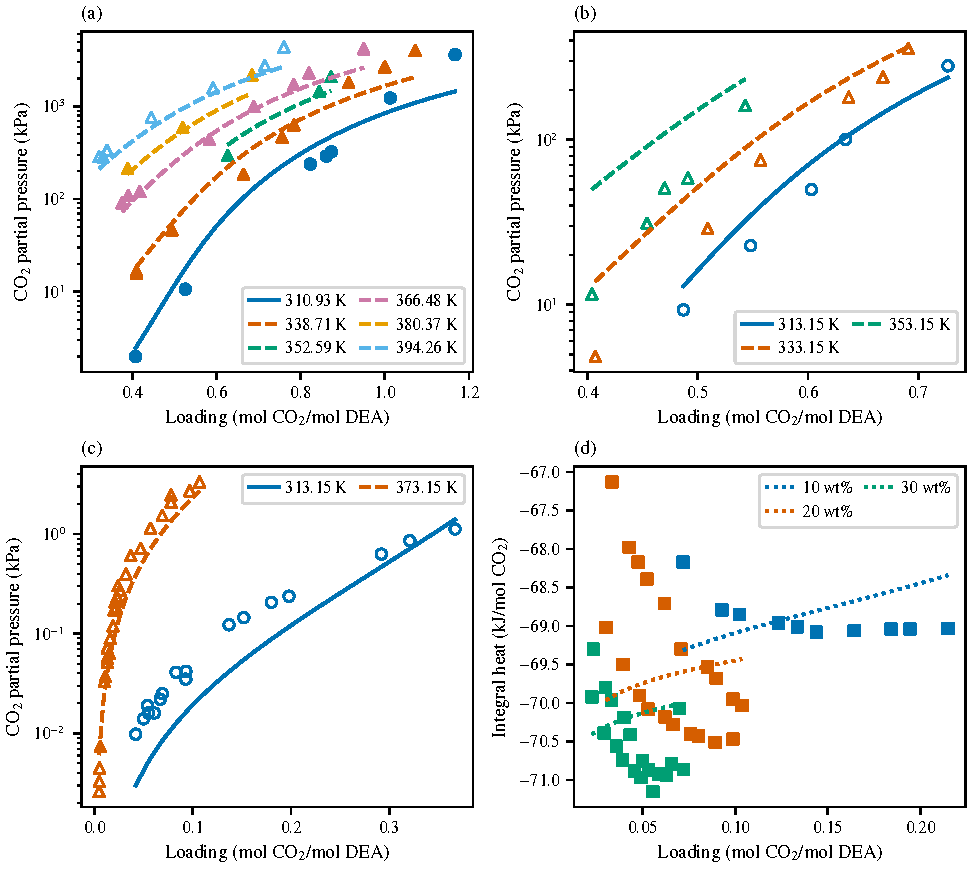
\includegraphics[width=0.85\linewidth]{dea-current-measured-model.pdf}
\caption{Loaded aqueous DEA against loading: measurements (symbols; filled if fitted) and the DEA model (lines). \COtwo partial pressures of Lawson and Garst \cite{lawsonGasSweeteningData1976} (a), Seo and Hong \cite{seoSolubilitiesCarbonDioxide1996} (b) and Lal et al.\ \cite{lalSolubilityH2SCO21985} (c), and integral absorption heats of Carson et al.\ \cite{carsonEnthalpySolutionCarbon2000} (d). Symbol shapes identify the temperature, and the colors the curves of each panel, which in (d) differ in DEA content. Solid lines lie inside the measured temperature ranges of both R4 and R5, dotted lines outside the R4 range only and dashed lines outside both.}
\label{fig:dea-pressure}
\end{figure}

% P:transfer-dea-binary
The water--DEA binary is a negative result.
The water--DEA interaction is a constant fitted beforehand to the 42 bubble pressures of Horstmann et al.\ at \SI{365.15}{\kelvin} \cite{horstmannPhaseEquilibriumExcess2002}, which it describes with an AARD of 0.8\,\%, but the calculated excess enthalpies are positive where the 14 measured ones are negative.
A second fit, made with the MEA-fitted shared set, gave the interaction a temperature coefficient and fitted it to all three binary data sets; the excess enthalpies then agree far better, but the bubble pressures and, after the same reactive fit, the \COtwo partial pressures outside the fit agree worse (Section~\ref{supp-sec:s-dea-binary}).
With the adopted DEA pure-component and association parameters, neither of the two fits represents the binary excess enthalpies and bubble pressures together, and the DEA model keeps the constant interaction.

\subsubsection{MDEA}\label{sec:results-mdea}
% P:transfer-mdea-fit
The MDEA model fits eight parameters, among them the MDEA--water interaction, which is part of the reactive fit.
The 66 fitted total pressures of Kuranov et al.\ \cite{kuranovSolubilitySingleGases1996} deviate by 10.1\,\% (\cref{fig:mdea-pressure}).
Above the measured R5 range, from \SI{368}{\kelvin}, the 29 fitted pressures have an AARD of 12.5 and bias of 11.3\,\%, so most of them are overpredicted.
The fitted MDEA properties other than the loaded-solution pressures deviate by 0.1--13.9\,\%, and every fitted species ratio is overpredicted.
The loaded-solution pressures carry little weight in this fit: they contribute 1\,\% of the objective, and a refit of this model with other weights has not been made.

% P:transfer-mdea-outside
Outside the fit the agreement is uneven.
The 11 total pressures of Kuranov et al.\ at \SI{413}{\kelvin} deviate by 3.1\,\%, but the 101 \COtwo partial pressures of Ermatchkov et al.\ \cite{ermatchkovSolubilityCarbonDioxide2006}, at lower loadings and pressures, deviate by 38.4\,\% and are almost all underpredicted.
At 60 wt\% MDEA, above the fitted contents of 30--50 wt\%, the densities and heat capacities of Weiland et al.\ \cite{Weiland1998,weilandHeatCapacityAqueous1997} deviate several times more than at the fitted contents (Table~\ref{supp-tab:supplement-transfer-data}).

% P:transfer-mdea-parameters
The temperature coefficient of the MDEA--water interaction has a small standard error, and the interaction itself is held at its bound at \SI{423}{\kelvin} (\cref{sec:methods-phase}).
The cation--bicarbonate interaction is at its upper bound, the cation--water interaction is not distinguishable from zero, and the cation dispersion energy has a standard error of 9\,\% of its value (\cref{tab:transfer-fitted}).

\begin{figure}[pos=!tbp]
\centering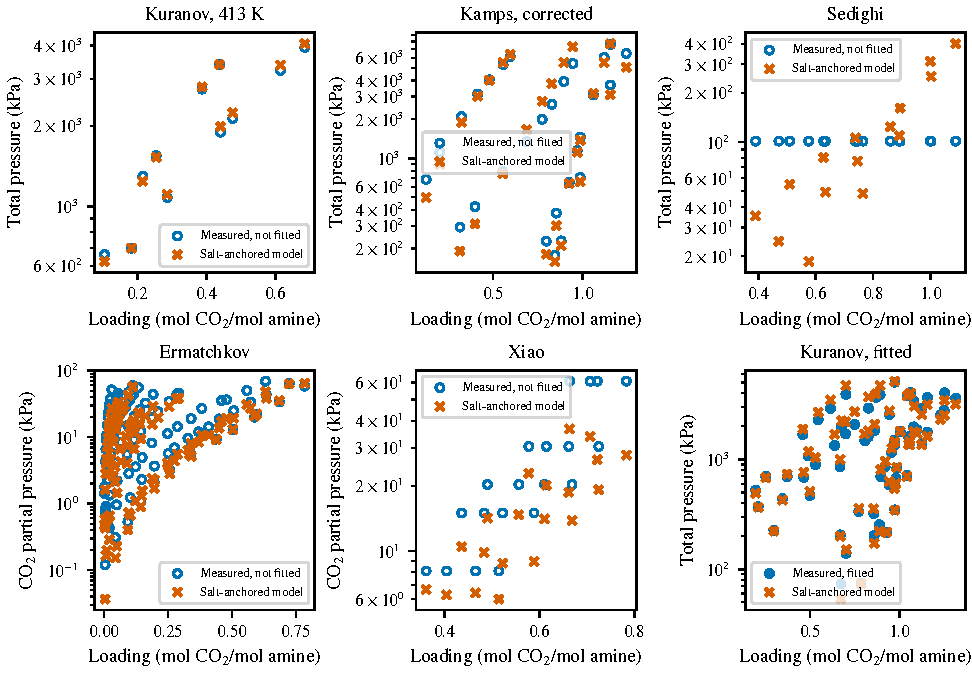
\includegraphics[width=0.9\linewidth]{mdea-current-measured-model.pdf}
\caption{Loaded aqueous MDEA against loading: measurements (circles; filled if fitted) and the MDEA model at each measured state (crosses). Total pressures of Kuranov et al.\ \cite{kuranovSolubilitySingleGases1996} at \SI{413}{\kelvin}, of P\'erez-Salado Kamps et al.\ at the temperatures corrected by Ermatchkov et al.\ \cite{ermatchkovSolubilityCarbonDioxide2006} and of Sedighi et al.\ \cite{sedighiExperimentalMeasurementThermodynamic2024} (upper row); \COtwo partial pressures of Ermatchkov et al.\ \cite{ermatchkovSolubilityCarbonDioxide2006} and of Xiao et al.\ \cite{xiaoCO2AbsorptionAqueous2018a}, and the fitted total pressures of Kuranov et al.\ (lower row). Each panel pools the temperatures and MDEA contents of its source.}
\label{fig:mdea-pressure}
\end{figure}

\subsubsection{AMP}\label{sec:results-amp}
% P:transfer-amp-fit
The AMP model fits nine parameters to 214 observations, among them all 105 loaded total pressures of Hartono et al.\ \cite{hartonoNewSolubilityHeat2021} and Tong et al.\ \cite{Tong2012} at 313--\SI{393}{\kelvin}.
These pressures deviate by 10.9\,\%, and the 51 \COtwo partial pressures of Kundu et al.\ \cite{kunduVaporLiquidEquilibriumCO22003}, which are not fitted, by 15.6\,\% (\cref{fig:amp-pressure}).
The fitted binary bubble pressures of AMP--water deviate by 1.1\,\%, and the fitted carbamate fractions have a larger deviation than the pressures but a small bias (Table~\ref{supp-tab:supplement-transfer-data}).

% P:transfer-amp-parameters
Two of the nine fitted AMP parameters are on bounds: the R4 enthalpy increment and the carbamate diameter, both at their lower bounds.
The fitted R4 correlation raises $\ln K_4$ at \SI{313.15}{\kelvin} by $0.389\pm0.230$, a factor of 1.475 in $K_4$.
The temperature coefficient of the \ce{AMPH+}--water interaction is $b_{\mathrm{AMPH^+,w}}=\SI{-52}{\kelvin}$, with a conditional standard error of \SI{63}{\kelvin}, so even the extended data do not distinguish it from zero; \cref{sec:results-phase} returns to this coefficient.

\begin{figure}[pos=!tbp]
\centering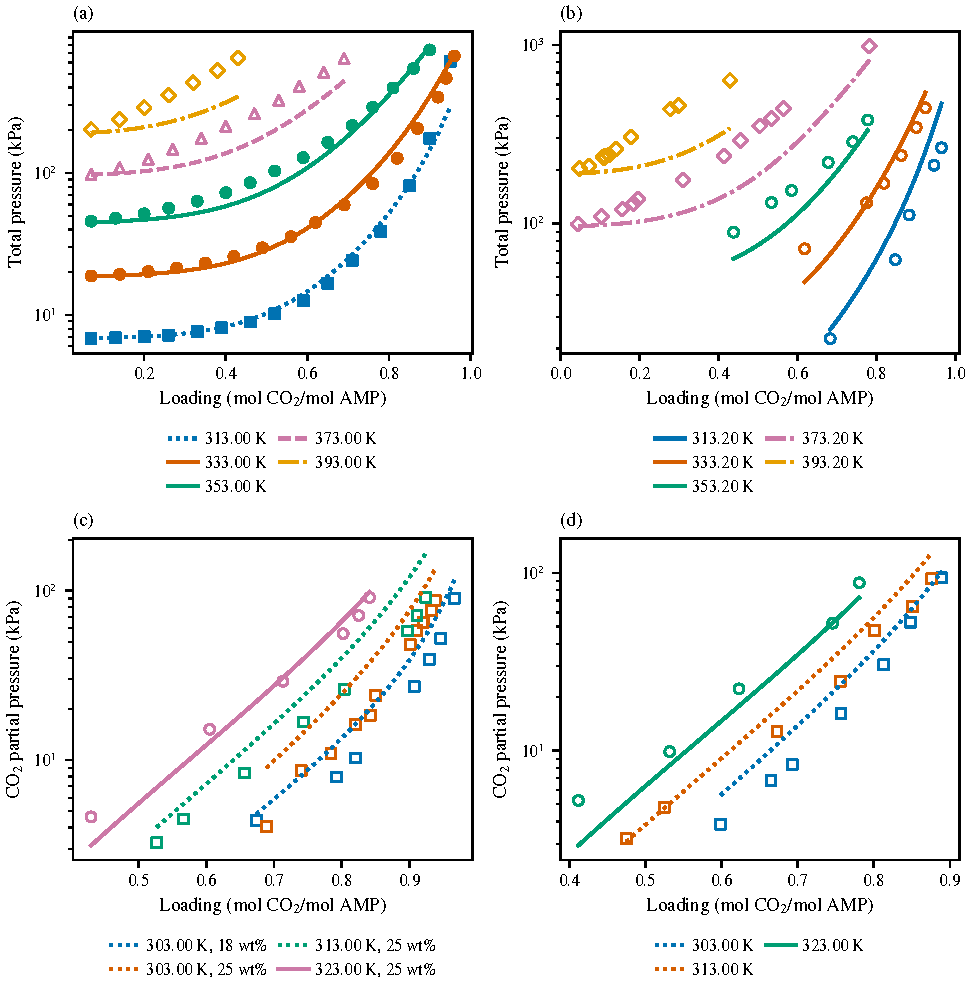
\includegraphics[width=0.85\linewidth]{amp-current-measured-model.pdf}
\caption{Loaded aqueous AMP against loading: measurements (circles; filled if fitted) and the AMP model at each measured state (crosses). Total pressures of Hartono et al.\ \cite{hartonoNewSolubilityHeat2021} at 313--\SI{353}{\kelvin} and at 373--\SI{393}{\kelvin} (upper row), total pressures of Tong et al.\ \cite{Tong2012} and \COtwo partial pressures of Kundu et al.\ \cite{kunduVaporLiquidEquilibriumCO22003} (lower row). Each panel pools the temperatures and AMP contents of its source.}
\label{fig:amp-pressure}
\end{figure}

\subsubsection{Effect of the salt-fitted shared interactions}\label{sec:results-shared}
% P:shared-tradeoff
\Cref{tab:amine-summary} sets the four models beside the same fits made with the MEA-fitted shared set, and Fig.~\ref{supp-fig:pressure-residuals} shows the pressure residuals of each model.
The fitted loaded-solution pressures are not one quantity across the amines: they are \COtwo partial pressures for MEA and DEA and total pressures for MDEA and AMP.
Fixing the two water--anion interactions from the salt data helps one amine and costs another.
For MDEA the deviation of the 66 fitted total pressures falls from 20.1 to 10.1\,\%, while that of the 101 \COtwo partial pressures of Ermatchkov et al., which are not fitted, rises from 17.9 to 38.4\,\%.
For DEA the deviation of the 30 fitted \COtwo partial pressures rises from 28.5 to 36.6\,\%.
For MEA and AMP the fitted pressures change by less than 0.3 percentage points, and the MEA pressures at \SI{393}{\kelvin} deteriorate (\cref{sec:results-restrictions}).

% P:shared-reading
No shared set is better for all four amines.
The salt-fitted interactions are adopted because data without an amine determine them, not because the amine data are fitted better.
MDEA responds most because it forms no carbamate: bicarbonate is its main product, so the water--bicarbonate interaction acts on its pressures directly, whereas in the MEA fit the carbamate and cation parameters compensate a change of that interaction.
A separate test agrees with this reading: with the MEA-fitted shared set, lowering the constant water--bicarbonate interaction from 0.765 to 0.1325 also lowered the deviation of the 66 fitted MDEA total pressures, to 11.2\,\%, and raised that of the \COtwo partial pressures outside the fit (Section~\ref{supp-sec:s-shared}).
How the MDEA fit changes when the shared parameters are released and fitted together with it remains to be tested.

\begin{table}[pos=!htbp]\small\setlength{\tabcolsep}{2pt}\caption{The four models: fitted parameters, pressure deviations and predicted liquid--liquid splits.}\label{tab:amine-summary}
\begin{tabular}{@{}>{\raggedright\arraybackslash}p{0.09\linewidth}>{\raggedright\arraybackslash}p{0.09\linewidth}>{\raggedright\arraybackslash}p{0.07\linewidth}>{\raggedright\arraybackslash}p{0.17\linewidth}>{\raggedright\arraybackslash}p{0.12\linewidth}>{\raggedright\arraybackslash}p{0.2\linewidth}>{\raggedright\arraybackslash}p{0.17\linewidth}@{}}
\toprule Model & Fitted parameters & On bounds & Fitted loaded-solution pressures\textsuperscript{a} & All fitted pressures\textsuperscript{b} & Pressures not fitted\textsuperscript{c} & Measured states with a liquid--liquid split\textsuperscript{d} \\ \midrule
MEA & 11 & 2 & $p_{\COtwo}$: $11.34$ (47) & $11.34$ (47) & $p_{\COtwo}$: $34.39$ (205) & 0 of 321 \\
DEA & 6 & 0 & $p_{\COtwo}$: $14.71$ (58) & $14.71$ (58) & $p_{\COtwo}$: $68.99$ (39) & 0 of 335 \\
MDEA & 8 & 1 & $P$: $4.44$ (66) & $3.34$ (131) & $P$: $29.96$ (54); $p_{\COtwo}$: $27.37$ (121) & 0 of 1564 \\
AMP & 9 & 2 & $P$: $10.82$ (105) & $8.89$ (131) & $P$: $3.86$ (5); $p_{\COtwo}$: $15.64$ (51) & 0 of 270 \\
\bottomrule\end{tabular}
\par\smallskip{\footnotesize\raggedright Pressure columns: AARD (Eq.~\eqref{eq:aard}) in \%, with the number of observations $N$ in parentheses. \textsuperscript{a}Fitted \COtwo partial pressures ($p_{\COtwo}$) of loaded MEA and DEA and fitted total pressures ($P$) of loaded MDEA and AMP. \textsuperscript{b}Column a with the fitted \COtwo-free bubble pressures of MDEA--water and AMP--water; neither column includes the fitted \COtwo--water pressures of Kiepe et al.\ in the MEA objective (Table~\ref{tab:mea-data}). \textsuperscript{c}MEA: all pressures not fitted, those at nominal 30 wt\% of the six sources of Table~\ref{tab:mea-data}, those of Wagner et al.\ and those at 15 and 45 wt\%; MDEA and AMP: total pressures and \COtwo partial pressures separately, the AMP total pressures including the 5 \COtwo-free bubble pressures of Tong et al. \textsuperscript{d}Number of measured states at which the model predicts a liquid--liquid split, of the measured states searched; no model has a detected instability at its grid states (Section~\ref{sec:results-phase}).\par}\end{table}


\FloatBarrier
\subsection{Phase stability}\label{sec:results-phase}
% P:phase-mea-dea
The searches are an endpoint check on each fitted model, separate from its optimization, and they are finite (\cref{sec:methods-phase}).
The MEA model shows no detected instability at any of the 2484 liquid states or 162 liquid--vapor states searched, and every search finished; B\"ottinger et al.\ observe a homogeneous liquid in their measured subset of loaded MEA solutions \cite{Bottinger2008}.
For DEA, 1269 of the 1271 searches finish, none with a detected instability; the other two did not finish and are not counted as stable (Section~\ref{supp-sec:s-phase}).

% P:phase-mdea-binary
For MDEA the result depends on the conditions.
In the \COtwo-free solution the bound of \cref{sec:methods-phase} keeps the MDEA--water interaction below the calculated onset of a liquid--liquid gap at each of the 33 tested temperatures (\cref{fig:mdea-gap-onset}).
The bound suppresses the gap only through the tested temperatures: with the fitted temperature law extrapolated, the gap first appears between 423.150 and \SI{423.156}{\kelvin} at \SI{1.466}{\mega\pascal}, so the MDEA model must not be used above about \SI{423}{\kelvin}.
No measurement of liquid--liquid coexistence in this system was used.

\begin{figure}[pos=!htbp]
\centering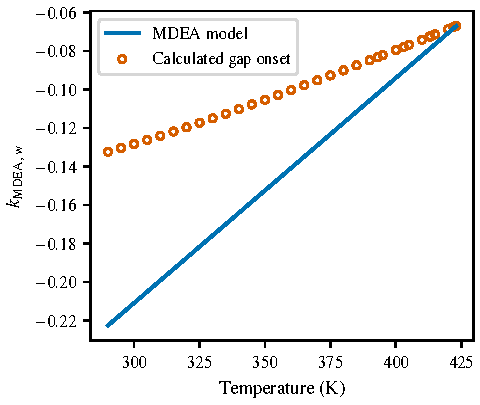
\includegraphics[width=0.5\linewidth]{mdea-gap-onset.pdf}
\caption{MDEA--water interaction $k_{\mathrm{MDEA,w}}$ against temperature at \SI{1.466}{\mega\pascal}: the MDEA model (solid line), the fit with the MEA-fitted shared set (dashed line, nearly coincident) and the smallest tested value at which a liquid--liquid gap appears in the calculated \COtwo-free MDEA--water solution (open circles), at 33 temperatures from 290 to \SI{423}{\kelvin}. A gap appears where the interaction exceeds the onset value; the bound at \SI{423}{\kelvin} is set $10^{-4}$ below the largest tested value without a gap.}
\label{fig:mdea-gap-onset}
\end{figure}

% P:phase-mdea-loaded
Of the \num{11824} MDEA searches, 1248 did not finish, 1024 with a bubble reference refusal, that is, at grid states where no bubble pressure could be calculated, and 222 of them at measured states.
The searches that finish detect an instability at 26 distinct states.
At 25 of them a density, a species fraction or an absorption heat was measured, and the instability is toward a dilute phase of gas-like density: the pressure assigned to the calculation, 0.100--\SI{4.190}{\mega\pascal}, lies below the calculated bubble pressure, so the values calculated there refer to a liquid that the model does not predict to be stable.
No second liquid is confirmed at any of these 25 states.
The remaining state is a confirmed liquid--liquid split at a grid state far outside the measured conditions: \SI{383.15}{\kelvin}, 78.6 wt\% MDEA, a loading of 1.368 mol/mol and \SI{121.3}{\mega\pascal} (Section~\ref{supp-sec:s-phase}).
The MDEA model is therefore not free of calculated splits, and 222 of its 1564 searches at measured states give no result.

% P:phase-amp
For AMP, all 666 searches of the AMP model finish without a detected instability, also when the trial compositions of earlier searches are tested.
This was not so for the first AMP fit.
That fit, made with the MEA-fitted shared set, used only the 47 loaded total pressures of Hartono et al.\ at 313--\SI{353}{\kelvin}, from which it deviates by 10.3\,\%, and it gave $b_{\mathrm{AMPH^+,w}}=\SI{-219}{\kelvin}$ with a conditional standard error of \SI{81}{\kelvin}.
Its searches gave 73 confirmed liquid--liquid splits and 20 further detected instabilities among the same 666 states, all of them at 363--\SI{393}{\kelvin}, above its fitted pressures (\cref{fig:amp-splits}).
At 373--\SI{393}{\kelvin} it underpredicted every measured total pressure of Hartono et al.\ and of Tong et al., by 28.1 and 25.3\,\% on average.

% P:phase-amp-refit
Fitting those measured pressures removed the splits.
With the 58 further pressures in the objective and the same shared set, the coefficient becomes \SI{-181}{\kelvin}, the pressures at 373--\SI{393}{\kelvin} of Hartono et al.\ deviate by 6.7\,\%, and no search detects an instability; the same holds for the AMP model, which also has the salt-fitted interactions.
The splits were therefore a consequence of extrapolating a weakly determined temperature coefficient beyond the fitted pressures, not a property that the AMP data support.
In the first fit that coefficient raised the cation--water interaction from $-0.178$ at \SI{353}{\kelvin} to $-0.115$ at \SI{393}{\kelvin}, and with the weaker cation--water attraction an ion-rich second liquid lowered the Gibbs energy; in the AMP model the interaction changes only from $-0.202$ at \SI{353}{\kelvin} to $-0.187$.
Neither Hartono et al.\ nor Tong et al.\ report the phase state of their samples, and no measurement of liquid--liquid coexistence in loaded aqueous AMP was used, so the single liquid of the AMP model is consistent with the data but not established by them.

\begin{figure}[pos=!htbp]
\centering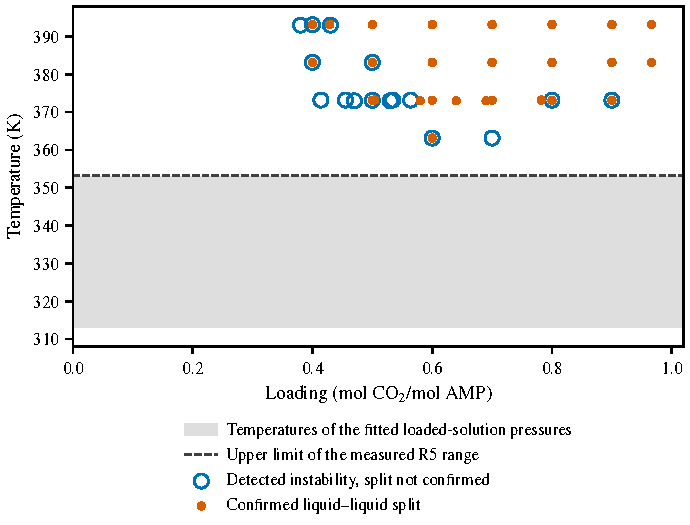
\includegraphics[width=0.72\linewidth]{amp-splits.pdf}
\caption{Searched states at which the first AMP fit, made with only the loaded total pressures at 313--\SI{353}{\kelvin}, has a detected instability toward a second liquid: the 73 with a split confirmed by a two-liquid equilibrium calculation and the 20 at which that calculation did not return two distinct liquids. The AMP model, which also fits the pressures at 373--\SI{393}{\kelvin}, has none. States at different AMP contents and pressures can project onto one point; states without a detected instability are not drawn. Shaded band: temperatures of the loaded-solution pressures in the first fit; dashed line: upper limit of the measured R5 range; plus signs: states of the measured total pressures of Hartono et al.\ and Tong et al.}
\label{fig:amp-splits}
\end{figure}

% P:phase-reading
The practical lesson is limited to this case: a phase-stability search showed where a fit had been extrapolated, at conditions where the deviations of its fitted data gave no warning.
Stability has been imposed during estimation for nonreactive binaries, where parameter sets fitted to vapor--liquid data alone are known to give false liquid--liquid splits \cite{mitsosBilevelOptimizationFormulation2009,bollasBilevelOptimizationFormulation2009,glassParameterEstimationCubic2018}; here it is checked after the fit, and for AMP the remedy was data, not a constraint.

\section{Discussion}\label{sec:discussion}
\subsection{Absorber and stripper temperatures}\label{sec:discussion-bands}
% P:results-temperature-bands
An absorber operates at about 313--\SI{353}{\kelvin} and a stripper at about 373--\SI{393}{\kelvin}, and the calibrations are not equally supported in the two ranges.
For MEA, the \COtwo partial pressures at 30 wt\% that are not fitted deviate by 27.25\,\% at 313--\SI{353}{\kelvin}, on 69 observations, and by 29.66\,\% at 373--\SI{393}{\kelvin}, on 66, each set including the pressures of Wagner et al.\ \cite{wagnerSolubilityCarbonDioxide2013} (Table~\ref{supp-tab:supplement-temperature-bands}).
At 373--\SI{393}{\kelvin}, where no loaded-solution observation of MEA is fitted, the 15 heat capacities and 26 densities deviate on average by 1.2\,\% and 0.4\,\%.
The absorption heats at \SI{393}{\kelvin} are low by 5.8\,\% for Vinjarapu et al.\ \cite{HemaBhavya2025}, 10.0\,\% for Kim et al.\ \cite{Kim2014} and 13.4\,\% for Kim and Svendsen \cite{Kim2007} on average, so the calculated heat rises less with temperature than these calorimetric data show.

% P:discussion-bands-transfer
For the three further amines the support at stripper temperatures differs.
The AMP model fits loaded total pressures up to \SI{393}{\kelvin}.
The fitted MDEA pressures above \SI{368}{\kelvin} lie outside the measured R5 range and are mostly overpredicted.
For DEA, 23 of the 30 fitted pressures lie outside the measured temperature range of R4 and 23 outside that of R5 (Table~\ref{supp-tab:supplement-transfer-data}), and the isotherm at \SI{394}{\kelvin} is not fitted.

\subsection{Comparison with published models}\label{sec:results-literature}
% P:literature-mea
\Cref{tab:mea-data} and Table~\ref{supp-tab:supplement-mea-comparison} compare the MEA model with the model of Polley and Hedengren \cite{polleyReactiveEPCSAFTModeling2026}.
The MEA model agrees better on most pressure, species, density and heat-capacity sets but worse on the Aronu 45 wt\% pressures; the two models were fitted to different data, so these deviations do not rank them.
On the 19 \COtwo partial pressures of Ma'mun et al.\ near \SI{393}{\kelvin} (\cref{tab:published-models}), the MEA model deviates by 38.4\,\%, more than the PC-SAFT calculation of Baygi and Pahlavanzadeh, which fitted no ternary data, and the eNRTL model of Zhang et al., which fitted these pressures.
Hong et al.\ report 1.53\,\% for a pathway-weighted PC-SAFT model of loaded MEA \cite{hongModelingCO2Absorption2027}; that value is a deviation from the simulator pressures to which the model was fitted, with a pathway weight fitted at each state, not from measurements, and Section~\ref{supp-sec:s-hong} evaluates their parameters on the measured pressures.

\begin{table}[pos=!htbp]\small\setlength{\tabcolsep}{2pt}\caption{Pressure AARD of this work and of published models on observation sets that no listed model fitted or that every listed model fitted.}\label{tab:published-models}
\begin{tabular}{@{}>{\raggedright\arraybackslash}p{0.5\linewidth}S[table-format=2.2]@{}}
\toprule Observations and model & {AARD (\%)} \\ \midrule
\addlinespace\multicolumn{2}{@{}l}{\textit{Not fitted by any listed model}} \\*
Ma'mun et al.\ \cite{Mamun2005}, MEA $p_{\COtwo}$, 393 K (19) &  \\
\quad This work & 38.66 \\
\quad PC-SAFT \cite{Baygi2015} & 21.03 \\
\addlinespace[2pt]Ermatchkov et al.\ \cite{ermatchkovSolubilityCarbonDioxide2006}, MDEA $p_{\COtwo}$ (101) &  \\*
\quad This work\textsuperscript{b} & 29.23 \\
\quad Ermatchkov et al., set I \cite{ermatchkovSolubilityCarbonDioxide2006} & 16.8 \\
\addlinespace\multicolumn{2}{@{}l}{\textit{Fitted by every listed model}} \\*
Kuranov et al.\ \cite{kuranovSolubilitySingleGases1996}, MDEA $P$ (82)\textsuperscript{a} &  \\
\quad This work & 4.40 \\
\quad eNRTL \cite{zhangThermodynamicModelingCO22011} & 6.8 \\
\quad ePC-SAFT \cite{raeispourshiraziApplicationEPC_SAFTMBEoS2020} & 10.9 \\
\addlinespace[2pt]Tong et al.\ \cite{Tong2012}, AMP $P$ (\res{amp-assessment-tong-pressure-count-literature})\textsuperscript{a} &  \\*
\quad This work & \res{amp-reported-tong-total-pressure-aard-literature} \\
\quad eNRTL \cite{yiOpenAccessThermodynamically2024} & 8.0 \\
\quad eNRTL \cite{hartonoSolubilityCO201M2020} & 9.3 \\
\bottomrule\end{tabular}
\par\smallskip{\footnotesize\raggedright AARD follows Eq.~\eqref{eq:aard}; published values are those reported in each source; number of observations in parentheses. $p_{\COtwo}$: \COtwo partial pressure; $P$: total pressure; set I: the first of the two parameter sets of Ermatchkov et al. \textsuperscript{a}This work fitted 70 of the 82 and \res{amp-reported-tong-fitted-pressure-count-literature} of the \res{amp-assessment-tong-pressure-count-note}; the published Kuranov values are matched to the 82 by count. \textsuperscript{b}Used to choose the initial parameters.\par}\end{table}


% P:literature-mdea
For MDEA, \cref{tab:published-models} sets the MDEA model beside published values on three sets of observations.
On the 82 total pressures of Kuranov et al., of which the MDEA model fitted 70, it deviates by 8.8\,\%, between the two models that also fitted these pressures \cite{raeispourshiraziApplicationEPC_SAFTMBEoS2020,zhangThermodynamicModelingCO22011} and well below the ePC-SAFT calculations of Uyan et al.\ and Wangler et al., which fitted no parameter to the ternary system \cite{Uyan2015,Wangler2018}.
The published values are identified with these 82 observations by their count only (Section~\ref{supp-sec:s-published}).
On the 101 \COtwo partial pressures of Ermatchkov et al.\ the MDEA model deviates by 38.4\,\%, against 16.8\,\% for their parameter set I, which did not fit them either, so here a published model that fitted nothing to these data is closer.
On the 28 total pressures of P\'erez-Salado Kamps et al.\ the two published sets, both fitted to them, are far closer than the MDEA model, which was not.

% P:literature-amp-dea
For AMP, two eNRTL models were fitted to the pressures used here: Yi et al.\ report 15.4\,\% for the 51 \COtwo partial pressures of Kundu et al.\ and 8.0\,\% for the 45 total pressures of Tong et al.\ \cite{yiOpenAccessThermodynamically2024}, and Hartono et al.\ report 17.3 and 9.3\,\% \cite{hartonoSolubilityCO201M2020}.
The AMP model deviates by 15.6\,\% from the Kundu pressures, which it did not fit, and by 10.5\,\% from the 45 pressures of Tong et al., of which it fitted the 40 loaded ones.
For DEA no deviation of a published model on identical observations is available (Section~\ref{supp-sec:s-published}).
Rodr\'iguez et al.\ compare their SAFT-VR model with the MEA pressures of Jou et al.\ and the MDEA pressures of Kuranov et al.\ only graphically \cite{Rodriguez2012}.

\subsection{Physical interpretation}\label{sec:discussion-interpretation}
% P:interpretation-01
The transfer shows what the shared parameters carry.
Water, \COtwo and the inorganic ions can be held fixed while each further amine is fitted, but the amine-specific fits absorb part of what the shared parameters leave out.
DEA and AMP each need a fitted carbamate-hydrolysis correlation, in opposite directions, and the cation--bicarbonate interactions of MEA and MDEA both end at their upper bound.
Fitted values of this kind are effective, and they are conditional on the shared set: when the shared water--anion interactions changed, the fitted cation--water interaction changed from $-0.188$ to $-0.141$ for DEA and from $-0.379$ to $-0.221$ for AMP, in both cases by many standard errors.

% P:interpretation-mdea-binary
The MDEA--water bound points to a limitation of this parameterization.
With the adopted MDEA pure-component and association parameters and the starts tried, a fit without the bound converged inside a calculated liquid--liquid gap of the \COtwo-free solution, and with the bound the interaction sits $10^{-4}$ below the largest tested value without a gap at \SI{423}{\kelvin}.
The binary is therefore close to a calculated demixing at the upper temperatures of the fit, and the calculated activities of that solution near \SI{423}{\kelvin} should be read with caution.
The linear temperature law of this interaction lets one bound act where the gap first appears; it has no other physical basis.

% P:interpretation-02
The electrostatic terms carry choices that the data do not test.
For the chain cations the Born diameter is that of one segment, not the volume-equivalent diameter, and for all ions the solvation average runs over all components rather than over ions and solvents only \cite{Figiel2025}.
Tests of these choices, made with the MEA-fitted shared set, changed the fitted MDEA pressure deviation by up to 2.4 percentage points and did not remove the carbonate deficit of \cref{sec:results-pressure} (Section~\ref{supp-sec:s-carbonate}).
That deficit limits any use of the calculated carbonate concentrations.

\subsection{Scope and limitations}\label{sec:limits}
% P:limits-scope
The four models are calibrations, not independent tests: every observation was examined during development, and the calculated phase behaviors are not established by the measurements.
They are not a basis for absorber design.

% P:limits-shared
The shared water--anion interactions rest on a salt fit with two values on their bounds and a deviation of 5.1\,\% for sodium carbonate; its data end at \SI{318}{\kelvin}, so the linear laws are extrapolated to \SI{393}{\kelvin}.
Neither shared set was fitted jointly with the four amines, so agreement for one amine does not establish the shared parameters for another.

% P:limits-estimation
Every fit is a local solution from two or three starts, and sensitivity to other starting sets remains to be tested.
The weights are assigned and differ between the amines; the MDEA objective is dominated by the densities of the \COtwo-free solution.
The standard errors exclude model discrepancy and the uncertainty of the shared parameters.
The amine reaction correlations, R4 and R5, are evaluated outside their source temperature ranges for every amine, unlike R1--R3, and the R4 correlations of DEA and AMP are fitted.
The DEA model rests on one source of loaded pressures, measured with methane in the cell.

% P:limits-model
Several fitted values are effective rather than molecular.
The \MEAH--\MEACOO interaction lies on its lower bound, where it may stand in for ion pairing, which the model does not describe, and the large cation--\COtwo interactions of MDEA and AMP and the dispersion energy of \ce{MDEAH+} are not interpreted physically.
The DEA and MDEA cations are chains and the other amine ions single spheres.
The fixed carbamate inputs of AMP are those of the MEA fit with the MEA-fitted shared set and were not updated to the MEA model (Section~\ref{supp-sec:s-parameters}).
The permittivity correlation is used beyond its source data, and ions affect it only through the volume and the neutral amounts, with no dielectric decrement.

% P:limits-phase
Finite searches do not prove global phase stability, and the MDEA searches leave a tenth of their states undecided.
Equations of state of the SAFT family can predict phase behavior that depends on the formulation \cite{privatAreSafeResults2010,yelashGlobalInvestigationPhase2005,polishukNumericalPitfallsCharacteristic2010}, and in electrolyte models the Born term and the permittivity mixing rule change the calculated liquid--liquid equilibrium \cite{AscaniHeld2021,Yang2024}.
The calculated MDEA split and gap are predictions of the stated model, and no measurement used here tests them.
Missing pressure histories, inconsistencies between sources, omitted carrier gas, solid precipitation and, for MEA, omitted oxazolidone further limit interpretation.
